%checked by mark May 9th 2019
\section{Placement of Social Contacts}
\label{sec:contacts:placing}

In this work \cite{Nassani2017a}, we look into options of where to place the social contacts relative to the user. We test two options: 1) life-sized where social contacts are presented as human-size virtual avatars displayed around the viewer, 2) a miniature option where the social contacts are displayed on a table-top nearby the viewer. 

\begin{figure}[h]
    \centering
    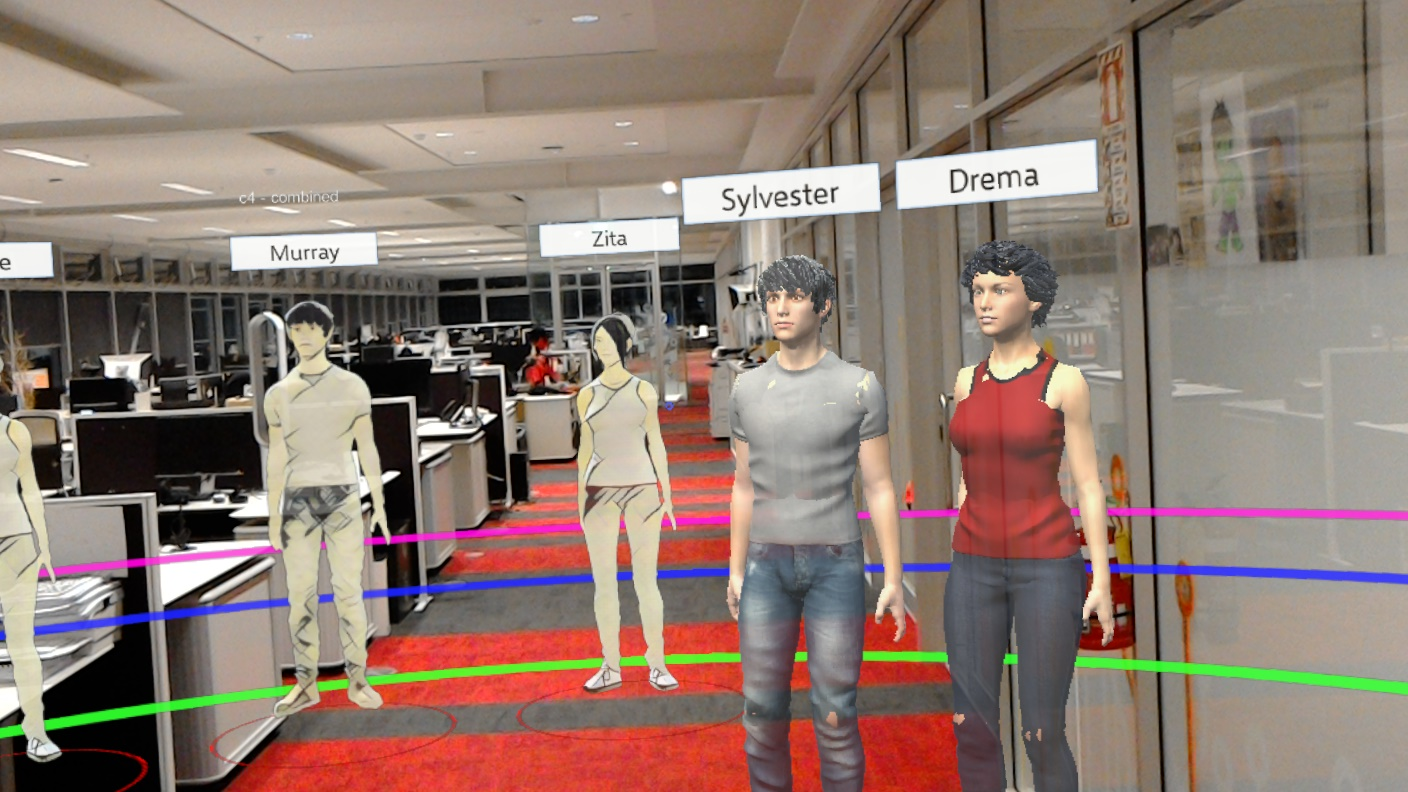
\includegraphics[width=.6\linewidth]{images/ismar17/20170625_205203_HoloLens.jpg}    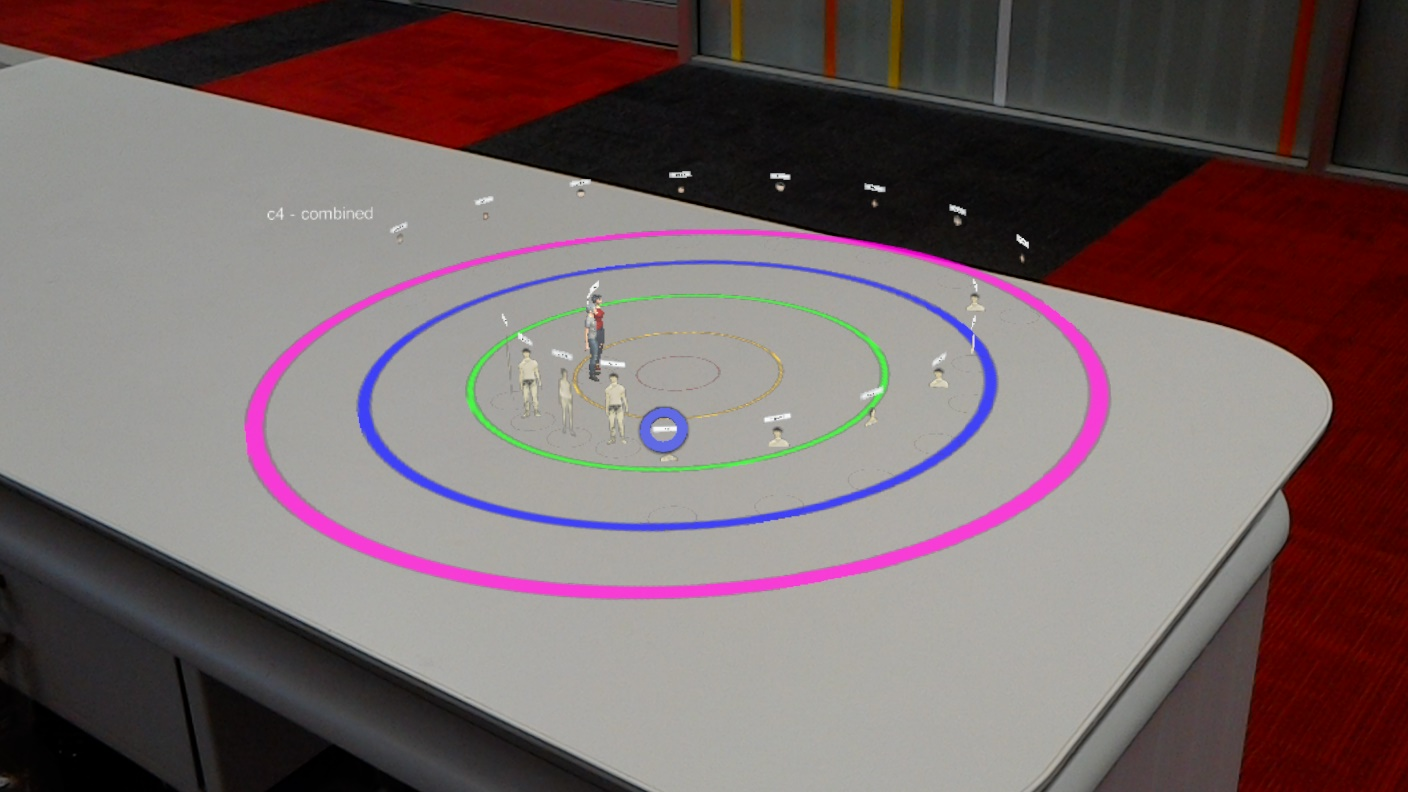
\includegraphics[width=.6\linewidth]{images/ismar17/20170625_205112_HoloLens.jpg}
    \caption{Prototype interfaces for contact placement. Life-sized (top) on the ground vs. Miniature (bottom) on a nearby surface.} 
    \label{fig:continuum:conditions}
\end{figure}

\subsection{Implementation}

We implemented a prototype (Figure \ref{fig:continuum:conditions}) on the Microsoft HoloLens to test two conditions on the contact placement dimension, one viewing avatars life-sized, and the other viewing avatars in miniature. The prototype also allowed the user (as a viewer) to select and move an avatar closer to or further away from the user position. The purpose of the selection and movement process is to change the social relationship between the viewer and their social contacts. 

\subsection{User Study}

We collected feedback from potential users during an open day at our lab as the participants tried demonstrations of the two conditions: C1-Life-sized (L) and C2-Miniature (M) representations of avatars. 

We collected feedback from 27 participants. On trying a demonstration of each condition, we asked participants to rate their experience on a 7-point Likert scale (where 1 = not very and 7 = very) for three subjective questions on: 

\begin{itemize}
    \item Q1: How easy was it to visualise social contacts?
    \item Q2: How natural was moving social contacts?
    \item Q3: How useful was this condition?
\end{itemize}

We also asked participants to think of situations where it would be useful to use each condition. Then we asked them to choose one of the conditions as the best condition based on their experience. 

\begin{figure}[h]
    \centering
    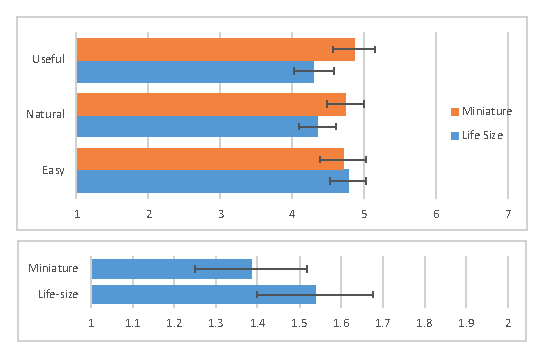
\includegraphics[width=.8\linewidth]{images/ismar17/images-09.eps}
    \caption{\textit{Top:} average results of subjective questions grouped by condition by question. \textit{Bottom:} average ranking results of preferred condition between Life-size and Miniature; 1=most preferred, 2=least preferred. Whiskers indicate standard error.}
    \label{fig:continuum:results}
\end{figure}

\subsection{Results}

The results of the questions (Figure \ref{fig:continuum:results}) did not show any statistically significant data for this user study. However, we did notice a trend for Natural and Usefulness favouring the Miniature condition over the Life-size condition. A Wilcoxon signed-rank test showed that using Life-Sized or Miniature did not elicit a statistically significant change in ease of use ($Z=-.529, p=.597$), natural interaction ($Z=-1.616, p=.106$), nor usefulness ($Z=-1.664, p=0.096$). 

Participants reported the most useful scenarios for the Life-size condition as \enquote{face-to-face conversations with a social contact} or \enquote{when zooming into a subset group of friends.} For the Miniature condition, participants reported \enquote{seeing the overall picture of social contacts} or \enquote{moving contacts between different social circles} as being useful. We also asked participants to rank the two conditions in terms of preference. Results (Figure \ref{fig:continuum:results}) show that more participants preferred the Miniature condition. A Wilcoxon signed-rank test showed that using Life-Sized or Miniature did not reach statistical significance ($Z=-.577, p=.564$).

%It would be good to include more discussion about the results from this user test
